% !TEX program = xelatex
\documentclass[12pt]{report}
\usepackage{fontspec}
\usepackage{polyglossia}
\usepackage[a4paper, top=1.5cm, bottom=1.5cm, left=3cm, right=3cm]{geometry}
\usepackage{listings}
\usepackage{tabularx}
\usepackage[ruled, vlined, linesnumbered]{algorithm2e}
\usepackage[table]{xcolor}
\newcommand\mycommfont[1]{\footnotesize\ttfamily\textcolor{gray}{#1}}
\SetCommentSty{mycommfont}

\definecolor{codegreen}{rgb}{0,0.6,0}
\definecolor{codegray}{rgb}{0.5,0.5,0.5}
\definecolor{codepurple}{rgb}{0.58,0,0.82}
\definecolor{backcolour}{rgb}{0.95,0.95,0.92}

\lstdefinestyle{mystyle}{
    backgroundcolor=\color{backcolour},   
    commentstyle=\color{codegreen},
    keywordstyle=\color{magenta},
    numberstyle=\tiny\color{codegray},
    stringstyle=\color{codepurple},
    basicstyle=\ttfamily\footnotesize, % Font chữ code nhỏ hơn text một chút
    breakatwhitespace=false,         
    breaklines=true,                 % Tự động xuống dòng nếu code quá dài
    captionpos=b,                    
    keepspaces=true,                 
    numbers=left,                    % Hiện số dòng bên trái
    numbersep=5pt,                  
    showspaces=false,                
    showstringspaces=false,
    showtabs=false,                  
    tabsize=4
}

\lstset{style=mystyle}

\lstset{
    basicstyle=\ttfamily\small,
    breaklines=true,
    frame=single,
    backgroundcolor=\color{gray!10},
    keywordstyle=\color{blue},
    commentstyle=\color{green!50!black},
    stringstyle=\color{red},
    numbers=left,
    numberstyle=\tiny,
}

\setdefaultlanguage{vietnamese}
\usepackage{graphicx}
\usepackage{fancyhdr}
\usepackage{amsmath}
\usepackage{tikz}
\usepackage[hidelinks]{hyperref}
\usepackage{booktabs}
\usepackage{float}
\usepackage{longtable}
\usepackage{indentfirst}

% Header & Footer
\pagestyle{fancy}
\fancyhf{}
\fancyhead[L]{BLOCKCHAIN}
\setlength{\headheight}{25pt}
\setlength{\headsep}{15pt}
\fancyhead[R]{\leftmark}
\fancyfoot[C]{\thepage}
\renewcommand{\sectionmark}[1]{\markboth{#1}{}}
\renewcommand{\thesection}{\arabic{section}}
\renewcommand{\thesubsection}{\thesection.\arabic{subsection}}
\renewcommand{\thefigure}{\arabic{figure}}
\renewcommand{\thetable}{\arabic{table}}

\begin{document}

\hypersetup{pageanchor=false}
% Trang bìa
\begin{titlepage}
    \centering
    \vspace*{1cm}

    \scalebox{0.9}{\Large \textsc{ĐẠI HỌC QUỐC GIA THÀNH PHỐ HỒ CHÍ MINH}}\\[0.2cm]
    {\large \textsc{TRƯỜNG ĐẠI HỌC KHOA HỌC TỰ NHIÊN}}\\[0.2cm]
    {\normalsize \textsc{KHOA CÔNG NGHỆ THÔNG TIN}}\\[0.5cm]
    \par\noindent\rule{\textwidth}{0.4pt}\par
    
\includegraphics[width=10cm]{img/Logo chinh.png}
    \par\noindent\rule{\textwidth}{0.4pt}\par
    \vspace{1.0cm}
    {\Huge \textbf{BÁO CÁO ĐỒ ÁN 01}}\\[0.5cm]
    %{\LARGE \textbf{Mã hóa dữ liệu trong suốt Transparent Data Encryption – TDE}}\\[1cm]


    {\large BLOCKCHAIN VÀ ỨNG DỤNG\\}
    {\large LỚP 23MMT}\\[0.8cm]

    \textbf{GIẢNG VIÊN}\\
    NGUYỄN ĐÌNH THÚC\\
    NGÔ ĐÌNH HY \\[2cm]
    \textbf{SINH VIÊN}\\
    NGUYỄN ANH KIỆT - 23127005\\
    PHAN THANH BÌNH - 23127028\\
    PHẠM VŨ NGỌC DUY - 23127183\\
    NGUYỄN TẤN PHƯỚC - 23127536\\
    NGUYỄN ĐẶNG MINH DUY - 23127042
    \vfill
    {\large \today}
\end{titlepage}

\clearpage
\hypersetup{pageanchor=true}

\pagenumbering{roman}
\tableofcontents
\clearpage
\pagenumbering{arabic}

% Các mục
%\section*{Bảng phân công công việc}
\addcontentsline{toc}{section}{Bảng phân công công việc}

\begin{table}[H]
    \centering
    \setlength{\tabcolsep}{10pt} % Tăng khoảng cách giữa chữ và viền
    \renewcommand{\arraystretch}{1.5} % Tăng chiều cao dòng cho thoáng
    \begin{tabular}{|c|l|c|p{6cm}|c|}
        \hline
        \textbf{STT} & \textbf{Họ và tên} & \textbf{MSSV} & \textbf{Nội dung thực hiện} & \textbf{Hoàn thành} \\ \hline
        1 & Nguyễn Anh Kiệt & 23127005 & Cài đặt SQL Server, quay video phần Cài đặt SQL Server, kết nối client, viết báo cáo & 100\% \\ \hline
        2 & Phan Thanh Bình & 23127028 & Cài đặt SQL Server, kết nối Client, quay video phần kết nối Client-Server, viết báo cáo & 100\% \\ \hline
        

    \end{tabular}
    \caption{Bảng phân công nhiệm vụ nhóm}
\end{table} 
\section{Cấu trúc thư mục}
\label{sec:project-structure}

Thư mục nộp \texttt{Lab01\_23127005\_23127028\_23127183\_23127536\_23127042} được viết gọn thành \texttt{Lab01\_<MSSV>/} dưới đây; chỉ liệt kê các thành phần chính.

\begin{lstlisting}[basicstyle=\ttfamily\footnotesize,numbers=none,caption={Cấu trúc thư mục nộp bài},label={lst:project-tree}]
Lab01_<MSSV>/
|-- src/
|   |-- main.py           # Chay mo phong
|   |-- configuration.py  # Doc, kiem tra cau hinh
|   |-- identities.py     # Nap danh tinh va khoa
|   |-- common.py         # Du lieu, ma hoa, hash, chu ky
|   |-- execution.py      # Thuc thi giao dich, state
|   |-- node.py           # Dong thuan, gossip, catch-up
|   |-- sim.py            # Mang, hang doi, dong ho ao
|   |-- byzantine.py      # Hanh vi tan cong
|   `-- validation.py     # Kiem tra ket qua mo phong
|-- config/               # default.json, identities.json
|-- tests/
|   |-- unit/             # Kiem thu thanh phan
|   |-- integration/      # Tich hop CLI va logging
|   |-- e2e/              # T1-T8 va kich ban mo rong
|   |-- regression/       # Ngan loi cu tai dien
|   |-- __main__.py       # Chay test, luu ket qua
|   |-- c_helpers.py      # Tao node va du lieu test
|   |-- event_logs.py     # Thu thap log tung test
|   |-- independent_oracle.py # Kiem chung doc lap
|   `-- test_mutation_gate.py # Test phat hien loi co y
|-- logs/                 # Log mo phong, test va console
|-- requirements.txt      # Phu thuoc cryptography
`-- README.md             # Huong dan cai dat va chay
\end{lstlisting}

\texttt{src/main.py} chạy mô phỏng qua \texttt{python -m src.main}; \texttt{tests/\_\_main\_\_.py} chạy kiểm thử qua \texttt{python -m tests -v}. Ba file hỗ trợ trong \texttt{tests/} lần lượt chuẩn bị dữ liệu, thu log và kiểm chứng ledger/state độc lập với các hàm xử lý trong \texttt{src/}.

Trong \texttt{logs/}, các nhóm \texttt{tests/}, \texttt{e2e/} và \texttt{t1-t8/} lưu từng lần chạy tại \texttt{run-*/}; mỗi run có \texttt{summary.json} và log từng test. Console ghi tổng số test, thời gian và kết quả; bằng chứng cụ thể được dẫn ở Mục~\ref{sec:testing}. Các lệnh cài đặt và chạy chi tiết nằm trong \texttt{README.md}.

\section{Giới thiệu}
\label{sec:introduction}

\subsection{Mục tiêu bài lab}
Bài lab yêu cầu xây dựng blockchain Layer 1 tối giản, nơi các validator dùng thông điệp có chữ ký qua mạng mô phỏng để thống nhất ledger và trạng thái, không cần cơ quan trung tâm. Với $n=3f+1$, tối đa $f$ validator Byzantine và mạng bán đồng bộ (độ trễ tối đa $\Delta$ sau GST), hệ thống phải giữ safety mọi lúc và bảo đảm liveness sau GST khi proposer trung thực được chọn và mạng ổn định trở lại.


\subsection{Các lựa chọn thiết kế chính}

Các lựa chọn thiết kế của hệ thống được tóm tắt như sau:
\begin{itemize}
    \item \textbf{Đồng thuận:} Dùng giao thức BFT với các bước \texttt{Propose}, \texttt{Prevote}, \texttt{Precommit} và \texttt{Commit}.
    \item \textbf{Mô phỏng mạng:} Dùng mô phỏng sự kiện rời rạc, hỗ trợ trễ, mất, nhân bản và đảo thứ tự thông điệp; seed cố định giúp tái lập các yếu tố ngẫu nhiên.
    \item \textbf{Xác thực thông điệp:} Dùng chữ ký Ed25519 và domain separation theo \texttt{TX:chain\_id}, \texttt{HEADER:chain\_id} và \texttt{VOTE:chain\_id} để ngăn giả mạo và tái sử dụng chữ ký sai ngữ cảnh.
    \item \textbf{Thực thi giao dịch:} Áp dụng giao dịch tuần tự, tất định trên state key--value; mỗi tài khoản chỉ được sửa namespace của mình và giao dịch phải có chữ ký, nonce hợp lệ.
    \item \textbf{Cam kết trạng thái:} Mã hóa dữ liệu theo dạng chuẩn rồi băm SHA-256, để các node xử lý cùng danh sách giao dịch theo cùng thứ tự sẽ tạo cùng state hash.
    \item \textbf{Truyền tải block:} Gửi header trước; chỉ gửi body sau khi node nhận chấp thuận header tương ứng.
    \item \textbf{Chịu lỗi Byzantine:} Mô phỏng node im lặng, equivocation, block không hợp lệ.
\end{itemize}

\section{Thiết kế hệ thống}
\label{sec:system-design}

\subsection{Kiến trúc tổng thể}

\begin{figure}[H]
\centering
\begin{tikzpicture}[x=1cm,y=1cm]
    \tikzstyle{layer}=[draw,rounded corners,align=center,text width=12.2cm,minimum height=1.2cm]
    \node[layer] (net) at (0,0) {\textbf{Tầng mạng / mô phỏng}\\Peer transport, gossip, REQUEST\_BODY, hàng đợi sự kiện, đồng hồ ảo, Send/Broadcast, Rate Limit, Peer Blocking};
    \node[layer] (cons) at (0,-2) {\textbf{Tầng đồng thuận}\\Proposer, bộ máy height--round, prevote/precommit, guard, timeout và lock};
    \node[layer] (exec) at (0,-4) {\textbf{Tầng thực thi}\\Kiểm tra transaction, nonce, namespace, cập nhật map key-value, tính state hash};
    \node[layer] (store) at (0,-6) {\textbf{Tầng lưu trữ / quan sát}\\Block, header, vote, commit certificate, ledger và log kiểm thử};
    \draw[->,thick] (net.south) -- (cons.north);
    \draw[->,thick] (cons.south) -- (exec.north);
    \draw[->,thick] (exec.south) -- (store.north);
\end{tikzpicture}
\caption{Kiến trúc phân tầng của simulator BFT}
\label{fig:architecture}
\end{figure}

\subsection{Mô hình dữ liệu}

Các cấu trúc dữ liệu chính của hệ thống gồm:
\begin{itemize}
    \item \textbf{Tx (Transaction):} Gồm \texttt{sender}, \texttt{nonce} để xác định thứ tự và chống phát lại, \texttt{key} và \texttt{value} để cập nhật dữ liệu, cùng \texttt{sig} xác thực giao dịch.
    \item \textbf{Header (Block Header):} Gồm \texttt{height}, \texttt{round}, \texttt{pol\_round}, \texttt{parent}, \texttt{state\_hash}, \texttt{tx\_root}, \texttt{proposer} và \texttt{sig}; các trường này xác định vị trí, nội dung cam kết và người đề xuất block.
    \item \textbf{Block:} Gồm \texttt{header} chứa metadata và các cam kết của block, cùng \texttt{txs} là danh sách giao dịch.
    \item \textbf{Vote:} Gồm \texttt{kind} (PREVOTE hoặc PRECOMMIT), \texttt{height}, \texttt{round}, \texttt{block\_hash}, \texttt{voter} và \texttt{sig} xác thực phiếu.
    \item \textbf{CommitCertificate:} Gồm \texttt{height}, \texttt{round}, \texttt{block\_hash} và các chữ ký PRECOMMIT của validator để xác minh quorum và việc commit.
    \item \textbf{SyncReq (Sync Request):} Gồm \texttt{requester}, \texttt{from\_height}, \texttt{to\_height}; trường \texttt{height} mặc định bằng 0 chỉ phục vụ ghi log.
    \item \textbf{SyncResp (Sync Response):} Gồm \texttt{responder}, \texttt{chain\_data} chứa các cặp block và CommitCertificate để đồng bộ, xác minh; trường \texttt{height} mặc định bằng 0 phục vụ ghi log.
    \item \textbf{State:} Gồm \texttt{data}, là bảng key--value của ứng dụng, và \texttt{nonces}, lưu nonce cuối của mỗi tài khoản để kiểm tra thứ tự và chống phát lại.
\end{itemize}



\subsection{Hệ thống mật mã}

\paragraph{Mã hóa dữ liệu (Encode).} Hàm \texttt{encode(o)} chuyển dữ liệu thành byte theo quy tắc thống nhất, có phân biệt kiểu và cấu trúc:
\begin{itemize}
    \item \texttt{None} được biểu diễn bằng byte định danh kiểu; \texttt{bool} bằng byte tương ứng với đúng hoặc sai.
    \item \texttt{int} được mã hóa thành 8 byte có dấu theo thứ tự Big-endian.
    \item \texttt{str} được mã hóa UTF-8; \texttt{bytes} và \texttt{bytearray} giữ nguyên nội dung.
    \item \texttt{list} và \texttt{tuple} mã hóa các phần tử theo thứ tự ban đầu.
    \item Các cặp trong \texttt{dict} được sắp xếp theo khóa trước khi mã hóa, giúp cùng dữ liệu luôn có cùng biểu diễn byte bất kể thứ tự chèn.
\end{itemize}
Quy tắc này tạo đầu vào nhất quán cho các thao tác băm và ký.
\paragraph{Hàm băm (Hash).} Hàm \texttt{H(data)} dùng SHA-256 và trả về digest 256 bit (32 byte). Hash block được tính từ bốn trường:
\begin{align*}
\mathrm{BlockHash} &= \operatorname{SHA256}(\operatorname{encode}([\texttt{height},\texttt{parent},\\
&\qquad\texttt{state\_hash},\texttt{tx\_root}])).
\end{align*}
Theo công thức này, \texttt{round}, \texttt{pol\_round}, \texttt{proposer} và \texttt{sig} không trực tiếp tham gia \texttt{BlockHash}; các header có cùng bốn trường trên sẽ có cùng hash dù các trường còn lại khác nhau.

\texttt{tx\_root} là SHA-256 của mã hóa danh sách giao dịch có thứ tự, mỗi phần tử gồm \texttt{[tx.body(), tx.sig]}; \texttt{tx.body()} chứa \texttt{sender}, \texttt{nonce}, \texttt{key} và \texttt{value}. \texttt{state\_hash} được tính từ \texttt{data} và \texttt{nonces} sau khi sắp xếp các phần tử rồi mã hóa. Trường \texttt{parent} liên kết block với block trước; thay đổi giao dịch hoặc trạng thái sẽ làm thay đổi các giá trị cam kết tương ứng.
\paragraph{Chữ ký số (Digital Signature).} \texttt{KeyPair} băm seed bằng SHA-256 để tạo khóa riêng Ed25519, rồi suy ra khóa công khai. \texttt{sign(kp, domain, body)} ký biểu diễn đã mã hóa của domain và nội dung; \texttt{verify(pk, domain, body, sig)} xác minh chữ ký với đúng khóa, domain và nội dung.

Domain separation dùng ngữ cảnh riêng theo loại thông điệp và chain:
\begin{itemize}
    \item \texttt{TX:chain\_id} cho giao dịch.
    \item \texttt{HEADER:chain\_id} cho header.
    \item \texttt{VOTE:chain\_id} cho phiếu.
\end{itemize}

\subsection{Cơ chế đồng thuận}

Quy trình trong 1 round: Propose (proposer xoay vòng) -> Prevote -> Precommit -> Finalize nếu được. Dưới đây là quy trình prevote và precommit.

    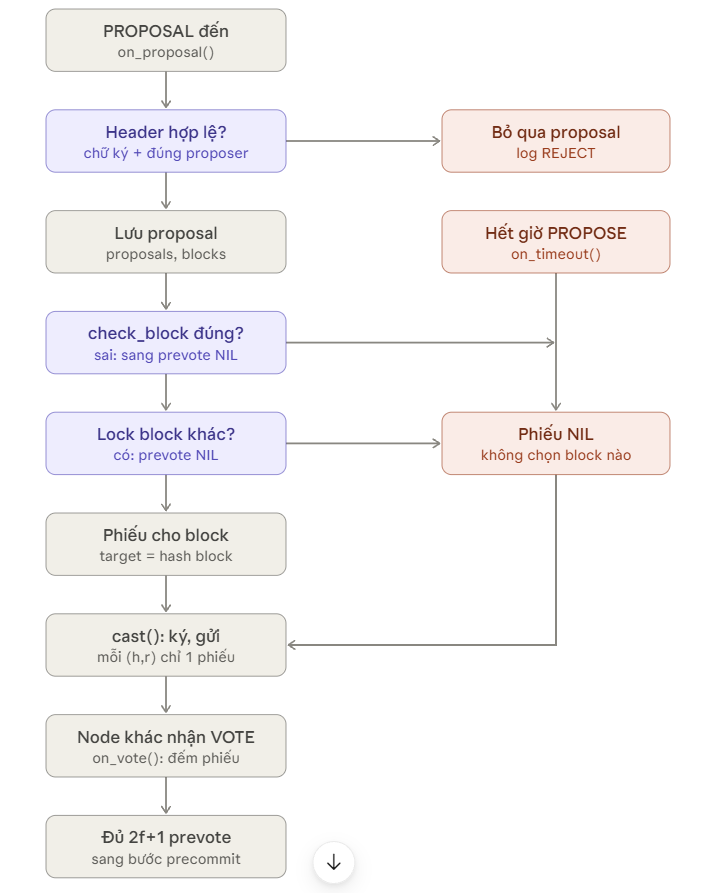
\includegraphics[width=0.45\textwidth,height=0.45\textheight,keepaspectratio]{prism-uploads/image_3.png}
    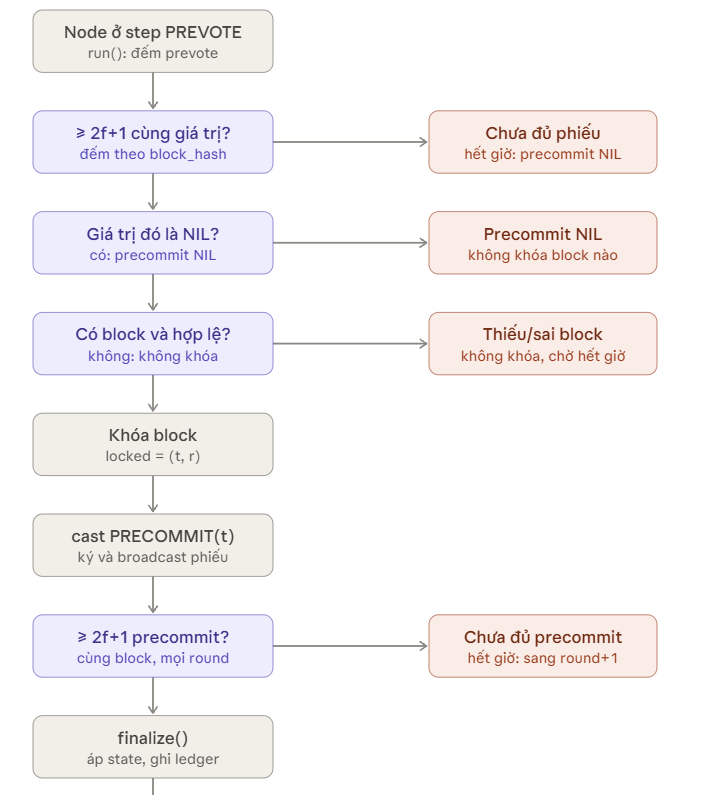
\includegraphics[width=0.45\textwidth,height=0.45\textheight,keepaspectratio]{prism-uploads/image.png}

\subsection{Đồng bộ catch-up}
\begin{figure}[H]
    \centering
    \begin{tikzpicture}[scale=0.8,x=1cm,y=0.85cm,transform shape,>=stealth,every node/.style={font=\small}]
        \tikzstyle{syncstep}=[draw,rounded corners,align=center,text width=7.2cm,minimum height=0.72cm,inner sep=3pt]
        \node[syncstep,fill=gray!10] (start) at (0,0) {Validator B bị chậm\\Height hiện tại = 7};
        \node[syncstep,fill=blue!6] (detect) at (0,-1.3) {Phát hiện validator A đã commit đến height 10};
        \node[syncstep,fill=gray!10] (request) at (0,-2.6) {Gửi \texttt{SYNC\_REQ}\\Yêu cầu height 8 đến 10};
        \node[syncstep,fill=gray!10] (receive) at (0,-3.9) {Validator A nhận yêu cầu};
        \node[syncstep,fill=gray!10] (headers) at (0,-5.2) {A gửi \texttt{SYNC\_HEADERS}\\Header kèm CommitCertificate};
        \node[syncstep,fill=blue!6] (verify) at (0,-6.5) {B xác minh header, chữ ký và certificate};
        \node[syncstep,fill=gray!10] (bodyrequest) at (0,-7.8) {B yêu cầu \texttt{REQUEST\_BODY}};
        \node[syncstep,fill=gray!10] (body) at (0,-9.1) {Nhận BODY / \texttt{SYNC\_RESP}};
        \node[syncstep,fill=blue!6] (check) at (0,-10.4) {Kiểm tra \texttt{tx\_root}, thực thi giao dịch\\và kiểm tra \texttt{state\_hash}};
        \node[syncstep,fill=blue!10] (decision) at (0,-11.7) {Dữ liệu hợp lệ?};
        \node[syncstep,fill=green!10] (ledger) at (-4.2,-13.2) {Có: cập nhật ledger};
        \node[syncstep,fill=red!10] (reject) at (4.2,-13.2) {Không: từ chối dữ liệu không hợp lệ};
        \node[syncstep,fill=gray!10] (continue) at (-4.2,-14.5) {Tiếp tục đồng bộ block còn thiếu};
        \node[syncstep,fill=green!10] (caughtup) at (-4.2,-15.8) {Bắt kịp blockchain};
        \draw[->] (start.south) -- (detect.north);
        \draw[->] (detect.south) -- (request.north);
        \draw[->] (request.south) -- (receive.north);
        \draw[->] (receive.south) -- (headers.north);
        \draw[->] (headers.south) -- (verify.north);
        \draw[->] (verify.south) -- (bodyrequest.north);
        \draw[->] (bodyrequest.south) -- (body.north);
        \draw[->] (body.south) -- (check.north);
        \draw[->] (check.south) -- (decision.north);
        \draw[->] (decision.south west) -- node[pos=0.5,above left]{Có} (ledger.north);
        \draw[->] (decision.south east) -- node[pos=0.5,above right]{Không} (reject.north);
        \draw[->] (ledger.south) -- (continue.north);
        \draw[->] (continue.south) -- (caughtup.north);
    \end{tikzpicture}
    \caption{Quy trình catch-up bằng header, certificate và body}
    \label{fig:catchup-headers-body}
\end{figure}
\subsection{Mô hình mạng mô phỏng}
Tầng mạng được triển khai trong \texttt{src/sim.py} thông qua lớp \texttt{Net}, theo mô hình mô phỏng sự kiện rời rạc (Discrete-Event Simulation). Các node trao đổi thông điệp bằng các hàm \texttt{send()} và \texttt{broadcast()}. Hàng đợi ưu tiên cùng đồng hồ ảo giúp mô phỏng có tính tất định.

\paragraph{Mô phỏng lỗi mạng.} Mạng hỗ trợ các lỗi trễ (Delay), mất gói (Drop), nhân bản (Duplicate) và đảo thứ tự (Reorder) theo xác suất cấu hình. Trước GST, mạng có thể không ổn định; sau GST, độ trễ truyền dẫn được giới hạn bởi $\Delta$, không tính thời gian chờ do giới hạn tốc độ gửi (Rate Limiting) hoặc chặn peer (Peer Blocking).

\paragraph{Giới hạn tốc độ gửi và chặn peer.} Hệ thống giới hạn số thông điệp gửi trên mỗi kết nối, trì hoãn các thông điệp vượt ngưỡng và hỗ trợ chặn hoặc bỏ chặn peer theo thời gian cấu hình.

\paragraph{Topology.} Hệ thống hỗ trợ cấu trúc full mesh hoặc danh sách liên kết tùy chỉnh, với độ trễ riêng cho từng liên kết thông qua \texttt{link\_delays}.

\paragraph{Ghi nhật ký mạng.} Hệ thống ghi nhận các sự kiện \texttt{SEND}, \texttt{DROP}, \texttt{DELAY}, \texttt{DUPLICATE}, \texttt{BLOCK} và \texttt{UNBLOCK}.
\subsection{Mô hình Byzantine}
\label{sec:byzantine-model}

Mỗi hành vi Byzantine là một lớp con của \texttt{Node} trong \texttt{src/byzantine.py}. Lớp con chỉ ghi đè đúng hàm cần làm sai; phần còn lại vẫn chạy như node trung thực. Ba nguyên tắc: (1) chỉ ký bằng khóa của chính nó, không giả chữ ký người khác; (2) chỉ tác động lên node khác qua mạng, không sửa trực tiếp dữ liệu của node khác; (3) cấu hình tấn công xong trước khi node bắt đầu chạy.

\begin{table}[H]
\centering
\small
\begin{tabularx}{\textwidth}{|p{3.5cm}|X|p{3.6cm}|}
\hline
\textbf{Lớp} & \textbf{Làm sai thế nào} & \textbf{Node trung thực chặn bằng} \\
\hline
\texttt{Silent} & Không gửi gì (chết hẳn), hoặc vẫn bỏ phiếu nhưng không đề xuất block. & Timeout rồi sang round mới. \\
\hline
\texttt{EquivocateVoter} & Ký hai phiếu khác nhau cho cùng (height, round, loại phiếu). & Chỉ đếm phiếu đến trước, log \texttt{EQUIVOCATION}. \\
\hline
\texttt{EquivocateProposer} & Đề xuất hai block hợp lệ khác nhau cho cùng (height, round). & Prevote block đến trước, log \texttt{EQUIVOCATION}. \\
\hline
\texttt{InvalidBlock} & Header ký đúng nhưng nội dung sai đúng một chỗ (parent, \texttt{tx\_root}, \texttt{state\_hash}, chữ ký tx, tx lặp, \texttt{pol\_round}). & Kiểm tra block, log \texttt{REJECT} đúng lý do, prevote NIL. \\
\hline
\texttt{Replay} & Gửi lại nguyên vẹn tin cũ (cùng chữ ký) sau một khoảng trễ. & Mỗi người chỉ một phiếu mỗi slot; tin quá cũ bị bỏ. \\
\hline
\texttt{ForkCoalition} & Cả nhóm Byzantine cùng ký cho hai block, gửi mỗi block cho một nửa mạng. & Chỉ dùng cho thí nghiệm $n=9$ ngoài giả định. \\
\hline
\end{tabularx}
\caption{Các hành vi Byzantine được mô phỏng}
\label{tab:byzantine}
\end{table}

Bật hành vi Byzantine bằng mục \texttt{"byzantine"} trong file cấu hình, ví dụ \texttt{\{"1": \{"behavior": "silent"\}\}}. Test nào dùng hành vi nào được nêu ở Mục~\ref{sec:testing}.

\section{Các vấn đề khi triển khai}
\label{sec:implementation}

\subsection{Các cơ chế bảo vệ (Guards)}.

Bảy luật tại mục 6.1 của đề bài được hiện thực như sau:

\small
\setlength{\tabcolsep}{3pt}
\begin{longtable}{|p{0.8cm}|p{7.0cm}|p{4.6cm}|}
\caption{Tóm tắt bảy luật đồng thuận và kiểm thử}\label{tab:consensus-guards}\\
\hline
\textbf{Luật} & \textbf{Cách kiểm tra và xử lý} & \textbf{Kiểm thử kiểm chứng} \\
\hline
\endfirsthead
\hline
\textbf{Luật} & \textbf{Cách kiểm tra và xử lý} & \textbf{Kiểm thử kiểm chứng} \\
\hline
\endhead
1 & Khóa slot \texttt{(height, round, PREVOTE)} trong \texttt{signed}; nếu đã ký thì không ký hash khác. & Gửi hai PREVOTE khác block cùng slot; chỉ một chữ ký được phát. \\
\hline
2 & Khóa riêng slot \texttt{(height, round, PRECOMMIT)}; \texttt{kind} tách slot này khỏi PREVOTE. & Yêu cầu hai PRECOMMIT khác block cùng slot; chỉ một chữ ký được phát. \\
\hline
3 & Kiểm tra height, parent, \texttt{tx\_root}, giao dịch, \texttt{state\_hash}, proposer và chữ ký Header; sai thì PREVOTE NIL. & Thử sai chữ ký, parent, giao dịch hoặc state hash; block bị từ chối. \\
\hline
4 & Đếm ít nhất $2f+1$ PREVOTE cùng block khác NIL rồi lưu block và round vào \texttt{locked}. & Cấp quorum $2f+1$; xác nhận \texttt{locked} được cập nhật. \\
\hline
5 & Đang khóa B, chỉ chuyển sang C khi có POL hợp lệ ở round cao hơn; proposer dùng POL cao nhất khi thích hợp. & Khóa B, cấp POL cho C ở round cao hơn; chỉ chuyển khi đủ điều kiện. \\
\hline
6 & Kiểm tra phase, chain, height/round và chữ ký trong domain \texttt{VOTE:chain\_id}; chữ ký ràng buộc các trường vote. & Gửi vote sai domain, chữ ký hoặc cửa sổ height/round; vote bị bỏ qua. \\
\hline
7 & \texttt{votes} chỉ đếm một vote mỗi voter/slot; vote lặp bị bỏ qua, hash khác ghi \texttt{EQUIVOCATION}. & Phát lại và gửi vote mâu thuẫn; không đếm trùng và có log equivocation. \\
\hline
\end{longtable}
\normalsize
\setlength{\tabcolsep}{6pt}


\subsection{Giao tiếp qua mạng}

Các validator lan truyền thông tin bằng gossip qua topology trong mạng mô phỏng ở \texttt{sim.py}, không phụ thuộc máy chủ trung tâm.

\subsubsection{Phát tán Header trước, Body sau}

Block proposal được truyền theo hai bước:
\begin{enumerate}
    \item Proposer tạo block, lưu phần thân giao dịch trong \texttt{self.bodies} và chỉ phát Header qua \texttt{send\_proposal()}.
    \item Validator nhận Header tại \texttt{on\_header()}, kiểm tra các trường có thể xác minh từ Header và chữ ký.
    \item Nếu chấp nhận Header, node gửi \texttt{REQUEST\_BODY} để lấy phần thân.
    \item Proposer xử lý yêu cầu tại \texttt{on\_request\_body()} và gửi Body tương ứng.
    \item Node nhận Body tại \texttt{on\_body()}, kiểm tra tính toàn vẹn và hợp lệ trước khi sử dụng.
\end{enumerate}
Tập \texttt{pending\_headers} lưu Header đã chấp nhận nhưng chưa có Body; \texttt{requested\_bodies} ngăn gửi lặp yêu cầu tải cùng một Body. Cách truyền này hạn chế tải dữ liệu không cần thiết vì node chỉ yêu cầu Body sau khi Header vượt qua bước kiểm tra ban đầu.


\subsubsection{Rate Limit và Peer Blocking}

Trong \texttt{sim.py}, giới hạn tốc độ gửi và cơ chế tạm khóa peer giúp hạn chế spam hoặc gửi quá nhiều thông điệp:
\begin{itemize}
    \item \textbf{Outbound rate limit:} \texttt{\_reserve\_send\_time()} dùng Sliding Window để xác định thời điểm gửi sớm nhất. Thông điệp vượt hạn mức được hoãn bằng sự kiện \texttt{SEND\_READY}.
    \item \textbf{Inbound peer throttling:} \texttt{\_receive()} đếm thông điệp từ từng peer trong cửa sổ thời gian; peer vượt ngưỡng bị tạm khóa.
    \item \textbf{Peer blocking:} \texttt{blocked\_peers} lưu peer bị khóa và thời điểm hết hạn.
    \item \textbf{Unblocking:} Sự kiện \texttt{UNBLOCK} được đưa vào hàng đợi; khi hết hạn, trạng thái chặn được gỡ và peer có thể gửi lại.
\end{itemize}
Các sự kiện \texttt{DELAY}, \texttt{BLOCK}, \texttt{DROP} và \texttt{UNBLOCK} được ghi log để kiểm tra hoạt động của cơ chế bảo vệ mạng.

\subsection{Cơ chế đồng thuận}

\subsubsection{Gossip giao dịch và Mempool}

Khi nhận giao dịch, \texttt{on\_tx()} kiểm tra định dạng, tính hash để loại giao dịch đã có trong \texttt{seen\_tx\_hashes}, xác minh tài khoản gửi và chữ ký Ed25519, rồi kiểm tra namespace theo dạng \texttt{sender/...}. Node cũng kiểm tra nonce không bị lặp hoặc cũ so với trạng thái hiện tại. Giao dịch hợp lệ được thêm vào \texttt{mempool} và phát tiếp tới các peer.

Khi tạo block, proposer chọn giao dịch trong mempool theo thứ tự \texttt{(sender, nonce)} và giới hạn số lượng bằng \texttt{max\_txs}. Cách sắp xếp này giúp các proposer lựa chọn giao dịch nhất quán hơn.

\subsubsection{Timeout và Round Skipping}

Timeout tăng dần theo round để tránh dừng khi proposer không hoạt động hoặc thông điệp bị mất:
\[
\operatorname{Timeout}(r)=\texttt{base\_timeout}+r\times\texttt{timeout\_inc}.
\]
Hàm \texttt{start\_round()} đăng ký timeout PROPOSE và timeout ROUND dự phòng. Khi timeout, node bỏ phiếu NIL hoặc bắt đầu round mới tùy trạng thái. Ngoài ra, \texttt{skip\_target()} xác định round cao nhất mà ít nhất $f+1$ validator khác nhau đã đạt tới. Nếu round này lớn hơn round hiện tại, \texttt{maybe\_skip\_round()} giúp node chuyển nhanh tới round mới thay vì tiếp tục chờ.

\subsubsection{Mở khóa bằng POL và đề xuất lại block}

Theo Luật 5, validator đang khóa block B không được tùy ý chuyển sang C; chỉ được chuyển khi quan sát POL hợp lệ cho C ở round cao hơn. Các hàm liên quan:
\begin{itemize}
    \item \texttt{on\_polka()} kiểm tra loại vote, height, round, block hash, voter duy nhất và chữ ký; chỉ chấp nhận khi có ít nhất $2f+1$ PREVOTE hợp lệ cho cùng block khác NIL.
    \item \texttt{best\_polka()} tìm POL hợp lệ ở round cao nhất nhỏ hơn round hiện tại, khi node đã có block tương ứng và block vượt qua \texttt{check\_block()}.
    \item \texttt{propose()} đề xuất lại block đã đạt POL thay vì tạo block mới, đồng thời ghi nhận \texttt{pol\_round}.
\end{itemize}

\subsection{Tính tất định của mô phỏng (Determinism)}

\begin{enumerate}
    \item \textbf{Đồng hồ ảo:} Mạng dùng \texttt{self.now} thay thời gian thực. Đồng hồ chỉ tiến khi mô phỏng lấy sự kiện kế tiếp ra xử lý, nên kết quả không phụ thuộc tốc độ máy hay thời gian hệ điều hành.
    \item \textbf{Sắp xếp trước khi duyệt:} Dictionary và tập hợp ảnh hưởng kết quả được duyệt theo thứ tự xác định bằng \texttt{sorted()}. Ví dụ, mempool theo \texttt{(sender, nonce)}, validator theo ID, và dữ liệu dùng tính hash được sắp trước khi mã hóa.
    \item \textbf{Khóa phụ \texttt{seq\_no}:} Hàng đợi heap \texttt{self.q} lưu sự kiện dạng
    \[
    (t,\ seq\_no,\ kind,\ src,\ dst,\ payload),
    \]
    trong đó \texttt{t} là thời điểm và \texttt{seq\_no} tăng dần khi thêm sự kiện. Khi nhiều sự kiện đồng thời, khóa này giữ thứ tự ổn định và tránh so sánh payload khác kiểu.
    \item \textbf{PRNG riêng và seed cố định:} Mạng dùng PRNG riêng khởi tạo từ seed cấu hình; mỗi node cũng có PRNG riêng nếu cần hành vi ngẫu nhiên. Tách PRNG tránh hoạt động của node này làm thay đổi chuỗi ngẫu nhiên của node khác.
\end{enumerate}

\section{Kiểm thử và kết quả}
\label{sec:testing}

\subsection{Thiết lập và kiểm thử thành phần}

Hình thức: sử dụng \texttt{unittest}, gồm unit test và mô phỏng E2E theo Mục 9 của đề bài. Cấu hình nền có $n=10$, $f=3$, quorum $Q=7$, seed 42 và mục tiêu tạo ra 5 block; mỗi ca thay đổi điều kiện mạng hoặc dữ liệu theo mục tiêu kiểm tra riêng. Safety được kiểm trên mọi height đã chốt của các node trung thực; progress được kiểm riêng bằng số block hoàn tất. Oracle độc lập xác minh ledger và trạng thái để tránh chấp nhận trường hợp các node cùng cho một kết quả sai.

\begingroup
\small
\setlength{\tabcolsep}{4pt}
\renewcommand{\arraystretch}{1.12}
\noindent\begin{tabularx}{\textwidth}{@{}>{\raggedright\arraybackslash}p{2.5cm}>{\raggedright\arraybackslash}X>{\raggedright\arraybackslash}p{4.4cm}@{}}
\toprule
\textbf{Nhóm kiểm thử} & \textbf{Ca kiểm và kỳ vọng} & \textbf{Kết quả thực chạy} \\
\midrule
Chữ ký và context & Nhận chữ ký đúng; loại chữ ký bị sửa, sai khóa, domain hoặc chain ID. & Đạt với TX, header, vote và certificate. \\
\addlinespace
Cập nhật state & Kiểm cập nhật hợp lệ, sai namespace, nonce cũ/nhảy cóc và hash ổn định khi đổi thứ tự map. & 6/6 ca executor đạt. \\
\addlinespace
Đếm vote & Vote trùng chỉ tính một lần; phát hiện vote mâu thuẫn cùng slot. & Đạt; vote trùng không tạo quorum. \\
\addlinespace
Xác thực block & Nhận proposal hợp lệ; loại header sai chữ ký, sai proposer hoặc state commitment. & Đạt; commitment sai bị chặn trước PREVOTE. \\
\bottomrule
\end{tabularx}
\endgroup

\subsection{Kết quả kiểm thử quy trình E2E theo kịch bản T1--T8}

Bảng~\ref{tab:test-matrix} gồm tám kịch bản bắt buộc, được chạy riêng ngày 06/11/2026: \textbf{20/20 test đạt trong 9,820 giây}, 0 failure/error/skip, exit code 0. T1--T8 là tám nhóm kịch bản, gồm lần lượt 1, 3, 1, 1, 2, 2, 4 và 6 test; không cộng riêng các biến thể subtest. Bằng chứng trong thư mục nộp: \texttt{logs/t1-t8/run-8rks9po9/summary.json}, các log từng test được liệt kê trong index và \texttt{logs/t1-t8-console.txt}. Trạng thái đạt dựa trên assertion và log xác nhận điều kiện thử đã xảy ra.

\begingroup
\small
\setlength{\tabcolsep}{4pt}
\renewcommand{\arraystretch}{1.12}
\begin{longtable}{@{}p{0.55cm}>{\raggedright\arraybackslash}p{3.15cm}>{\raggedright\arraybackslash}p{4.1cm}>{\raggedright\arraybackslash}p{6.2cm}@{}}
\caption{Đối chiếu kết quả T1--T8 với yêu cầu đề bài}
\label{tab:test-matrix}\\
\toprule
\textbf{ID} & \textbf{Điều kiện thử} & \textbf{Kỳ vọng } & \textbf{Kết quả quan sát} \\
\midrule
\endfirsthead
\toprule
\textbf{ID} & \textbf{Điều kiện thử} & \textbf{Kỳ vọng } & \textbf{Kết quả quan sát} \\
\midrule
\endhead
\bottomrule
\endfoot
T1 & Không lỗi; GST bằng 0, $\delta=1$; tắt duplicate/reorder và throttling. & Mọi node trung thực chốt cùng chain và state hash. & Đạt: Cả 10 node chốt đủ 5 block ở round 0; ba khóa tài khoản đều bằng \texttt{v5}, nonce đều bằng 5; state hash giống nhau. \\
\midrule
T2 & Duplicate 0,25; reorder 0,35; gửi vote trùng và mâu thuẫn cùng slot. & Không đếm trùng vote, không chốt block mâu thuẫn. & Đạt: Có DUPLICATE, DELAY; mỗi voter chỉ tính một lần; không fork sau khi thực hiện. \\
\midrule
T3 & Tiêm vote/header/TX sai chữ ký hoặc domain, cùng certificate giả. & Từ chối thông điệp và ghi lý do. & Đạt. Có \texttt{bad\_vote\_sig}, \texttt{bad\_header\_sig}, \texttt{bad\_tx\_sig} và \texttt{invalid\_cert\_sig}; dữ liệu giả không vào ledger; honest node vẫn chốt đủ 5 block. \\
\midrule
T4 & Gửi TX Alice nonce 1 hai lần trước commit và replay sau commit; chạy 3 height. & Giao dịch được áp dụng tối đa một lần. & Đạt. TX nằm đúng một lần trong ledger mỗi node; nonce Alice bằng 1, dữ liệu đúng đầu vào; mọi node chốt đủ 3 block, mempool cuối rỗng. \\
\midrule
T5 & Drop/delay trước GST; seed 42, 43, 44, 99; thêm biến thể drop 0,40. & Safety được giữ; không chốt hai block khác nhau tại cùng height. & 2/2 ca đạt, gồm các biến thể seed. Có DROP trước GST; không phát hiện conflicting finalization, certificate đã chốt hợp lệ. \\
\midrule
T6 & V1 im lặng; biến thể có V1, V4, V7 cùng im lặng. & Timeout kích hoạt, chuỗi tiếp tục tiến triển. & 2/2 ca đạt. Nhánh V1: V0 timeout PROPOSE tại $t=200$, chốt height 1 ở round 1 tại $t=788$ bởi proposer V2; mọi honest node chốt đủ 5 block. \\
\midrule
T7 & Proposer gửi proposal mâu thuẫn; tối đa $f=3$ Byzantine equivocate. & Không có conflicting finalization giữa các node trung thực. & 4/4 ca đạt. Có log tấn công và EQUIVOCATION; không fork; mọi honest node chốt đủ 5 block với certificate hợp lệ. \\
\midrule
T8 & Hai lần cùng seed, config và identity; thử thêm mạng lỗi và Byzantine. & Log giống từng byte và cùng final state hash. & 6/6 ca đạt, gồm đối chứng âm. Hai lần chạy hợp lệ đều hoàn tất, log gốc UTF-8 và final state hash bằng nhau trên mọi honest node; đối chứng sai bị phát hiện. \\
\end{longtable}
\endgroup

\subsection{Tổng kết và tái lập}

Chạy riêng toàn bộ nhóm \texttt{tests/e2e} ngày 06/11/2026 cho kết quả \textbf{37/37 test đạt trong 20,718 giây}, 0 failure/error/skip, exit code 0. Nhóm này gồm T1--T8 và các ca Byzantine, catch-up, mạng lỗi, ranh giới quorum. Bằng chứng: \texttt{logs/e2e/run-\_0c6h6zv/summary.json} và \texttt{logs/e2e-console.txt}. Thời gian này và thời gian riêng T1--T8 ở trên đều do \texttt{unittest} đo cho toàn bộ lần chạy tương ứng, không phải thời gian mô phỏng.

Lần chạy thử nghiệm trong thư mục nộp sử dụng Python 3.12.14 và \texttt{cryptography} 50.0.2. Kết quả: \textbf{150/150 test đạt}, 0 failure/error/skip, exit code 0, thời gian 35,265 giây; không cộng riêng các biến thể subtest. \\ Chạy lại từ thư mục nộp bài (thư mục có tiền tố \texttt{Lab01\_} tại gốc repository) bằng \texttt{python -X utf8 -B -m tests -v}. \\ Bằng chứng của lần chạy này nằm trong \texttt{logs/tests/run-4udyr5el/summary.json} và các log từng test được liệt kê trong đó; transcript \texttt{logs/acceptance-console.txt} ghi nhận tổng số test, thời gian và kết quả \texttt{OK} của cùng run. Các đường dẫn này được tính từ thư mục nộp bài; cách cài đặt và chạy chi tiết được trình bày trong README.

%% \section{Kết luận}
% \label{sec:conclusion}

% Bài lab đặt mục tiêu xây dựng simulator cho đồng thuận Byzantine hai pha, trong đó có mô hình mạng bán đồng bộ, chữ ký và hash có domain separation, kiểm tra transaction/state, luật quorum và hành vi Byzantine. Các mục trước đã mô tả kiến trúc, dữ liệu, guard, quy trình đồng thuận và kế hoạch kiểm thử để đối chiếu từng yêu cầu của đề.

% Bản báo cáo hiện chưa có mã nguồn, README hoặc log chạy trong workspace, vì vậy chưa thể kết luận các yêu cầu đã được hiện thực và kiểm chứng thành công. Trước khi nộp, nhóm cần cập nhật bảng T1--T8 bằng kết quả thật, xác nhận bảy luật theo mục 6.1 của đề, thay các ca bug minh họa bằng lỗi đã tái hiện (hoặc bỏ những ca không xảy ra), và ghi chính xác phiên bản Python/thư viện.

% \subsection{Hạn chế và hướng mở rộng}

% Các hướng mở rộng phù hợp gồm lưu bền ledger/lock/vote để restart an toàn; dùng Merkle tree nếu cần inclusion proof hoặc light client; tối ưu gossip và đo tải khi số validator tăng; và mở rộng mô hình membership, quản lý khóa, cũng như fault injection. Mỗi hướng cần được đánh giá cùng giả định an toàn và chi phí bổ sung, thay vì chỉ xem là cải tiến hiệu năng.
\section{Tài liệu tham khảo}
\label{sec:references}

\begingroup
\def\chapter#1#2{}

\begin{thebibliography}{99}

\bibitem{lamport-byzantine}
L. Lamport, R. Shostak, and M. Pease,
\newblock ``The Byzantine Generals Problem,''
\newblock \emph{ACM Transactions on Programming Languages and Systems}, vol. 4, no. 3, pp. 382--401, 1982.
\newblock DOI: \url{https://doi.org/10.1145/357172.357176}.

% \bibitem{dls-partial-synchrony}
% C. Dwork, N. Lynch, and L. Stockmeyer,
% \newblock ``Consensus in the Presence of Partial Synchrony,''
% \newblock \emph{Journal of the ACM}, vol. 35, no. 2, pp. 288--323, 1988.
% \newblock DOI: \url{https://doi.org/10.1145/42282.42283}.

% \bibitem{tendermint}
% E. Buchman, J. Kwon, and Z. Milosevic,
% \newblock ``The latest gossip on BFT consensus,'' 2018.
% \newblock \url{https://arxiv.org/abs/1807.04938}.

% \bibitem{castro-liskov-pbft}
% M. Castro and B. Liskov,
% \newblock ``Practical Byzantine Fault Tolerance,''
% \newblock in \emph{Proceedings of the Third Symposium on Operating Systems Design and Implementation (OSDI)}, 1999.
% \newblock \url{https://pmg.csail.mit.edu/papers/osdi99.pdf}.

% \bibitem{flp}
% M. J. Fischer, N. A. Lynch, and M. S. Paterson,
% \newblock ``Impossibility of Distributed Consensus with One Faulty Process,''
% \newblock \emph{Journal of the ACM}, vol. 32, no. 2, pp. 374--382, 1985.
% \newblock DOI: \url{https://doi.org/10.1145/3149.214121}.

% \bibitem{rfc8032}
% S. Josefsson and I. Liusvaara,
% \newblock \emph{RFC 8032: Edwards-Curve Digital Signature Algorithm (EdDSA)}, 2017.
% \newblock \url{https://www.rfc-editor.org/rfc/rfc8032}.

% \bibitem{nist-sha256}
% National Institute of Standards and Technology,
% \newblock \emph{FIPS PUB 180-4: Secure Hash Standard}, 2015.
% \newblock DOI: \url{https://doi.org/10.6028/NIST.FIPS.180-4}.

% \bibitem{cryptography-ed25519}
% The Python Cryptographic Authority,
% \newblock ``Ed25519 signing,'' \emph{Cryptography documentation}.
% \newblock \url{https://cryptography.io/en/latest/hazmat/primitives/asymmetric/ed25519/}.

% \bibitem{course-material}
% \textit{[Bổ sung tên môn học, tên giảng viên, tên đề bài/slide, đơn vị và năm học theo tài liệu nhóm thực sự sử dụng.]}

% \bibitem{ai-disclosure}
% \textit{[Nếu quy chế môn yêu cầu: khai báo công cụ AI đã sử dụng, mục đích sử dụng và phần nội dung có hỗ trợ; nhóm cần tự kiểm chứng mọi nội dung trong báo cáo.]}

\end{thebibliography}
\endgroup

%\bibliographystyle{plain}   % hoặc unsrt, alpha, ieee...
%\bibliography{references}   % tên file .bib (không cần .bib)

\end{document}